\documentclass[a4paper,12pt]{article}
\usepackage[english,ukrainian,russian]{babel}
\linespread{1}
\usepackage{ucs}
\usepackage[utf8]{inputenc}
\usepackage[T2A]{fontenc}
\usepackage[paper=portrait,pagesize]{typearea}
\usepackage{amsmath}
\usepackage{bigints}
\usepackage{amsfonts}
\usepackage{graphicx}
\usepackage{amssymb}
\usepackage{cancel}
\usepackage{gensymb}
\usepackage{multirow}
\usepackage{rotate} 
\usepackage{pdflscape}
\usepackage{bigstrut}
\usepackage[pageanchor]{hyperref}
\usepackage{chngpage}
\usepackage{fancybox,fancyhdr}
\newcommand\tab[1][1cm]{\hspace*{#1}}
\newcommand{\RomanNumeralCaps}[1]{\MakeUppercase{\romannumeral #1}}
\usepackage[left=20mm, top=20mm, right=15mm, bottom=15mm, nofoot]{geometry}


\begin{document}
    \pagestyle{fancy}
    \fancyhead{}
    \fancyhead[R]{ФІ-12 Завалій Олександр}
    \begin{center}
        \large{\textbf{Міністерство освіти і науки України\\
                Національний технічний університет України\\
                «Київський політехнічний інститут імені Ігоря Сікорського»\\
                Навчально-науковий Фізико-технічний інститут}}\\
        \hfill \break \hfill \break \hfill\break \hfill \break \hfill \break \hfill \break \hfill \break
        \hfill \break \hfill \break \hfill \break
        \begin{center}
            \normalsize{\textbf{ОПЕРАЦІЙНІ СИСТЕМИ\\
            Комп’ютерний практикум\\
            Робота №10}}
        \end{center}
    \end{center}
    \hfill \break \hfill \break \hfill \break \hfill \break \hfill \break \hfill \break \hfill \break
    \hfill \break \hfill \break \hfill \break \hfill \break 
    \begin{flushright}
        \large{ \hspace{35pt} Виконав:\\
            студент групи ФI-12\\
            Завалій Олександр\\} 
        \large{ \hspace{35pt} Перевірив:\\
        Кірієнко О.В.} 
    \end{flushright}
    \hfill \break \hfill \break \hfill \break \hfill \break \hfill \break \hfill \break \hfill \break
    \hfill \break
    \begin{center} \textbf{Київ-2023} \end{center}
    \thispagestyle{empty}

\newpage
    \begin{center}
        \section*{\bfseries{Робота №10.\\
        Інтерфейс файлової системи в ОС Linux }}
    \end{center}
    \textbf{Мета:} \\
    \hangindent=1.5cm 
    \hangafter=+1 \noindent
    Ознайомитися з реалізацією файлових систем в Linux і основними структурами даних, що використовуються віртуальною файловою системою
    (VFS). Дослідити механізм доступу до файлів через інтерфейс віртуальної файлової системи в Linux. \\
    \begin{center}
        \Large{Варіант №5}
    \end{center}
    Зміст індивідуального завдання: 

    Розробити програму, яка демонструвала б роботу ОС Linux при відкритті файлу процесом і читанні-записи в нього. При
    цьому досить показати тільки динаміку створення таблиць, пов'язаних з цією подією (таблиця дескрипторів файлу,
    таблиця відкритих файлів, масив файлових дескрипторів процесу). Наприклад, сценарій програми може бути таким:
    \begin{itemize}
        \item неявне відкриття стандартного файлу введення;
        \item неявне відкриття стандартного файлу виведення;
        \item неявне відкриття стандартного файлу виведення помилок;
        \item відкриття першого призначеного для користувача файлу;
        \item відкриття другого призначеного для користувача файлу;
        \item записування 20 байт в перший файл;
        \item зчитування 15 байт з другого файлу;
        \item записування 45 байт в перший файл. 
    \end{itemize}

    Після кожного з етапів друкуються таблиця дескрипторів файлів, таблиця відкритих файлів, таблиця відкритих файлів процесів.

\newpage
    \begin{figure}[h!]
        \begin{minipage}[h]{1\linewidth}
            \centering
            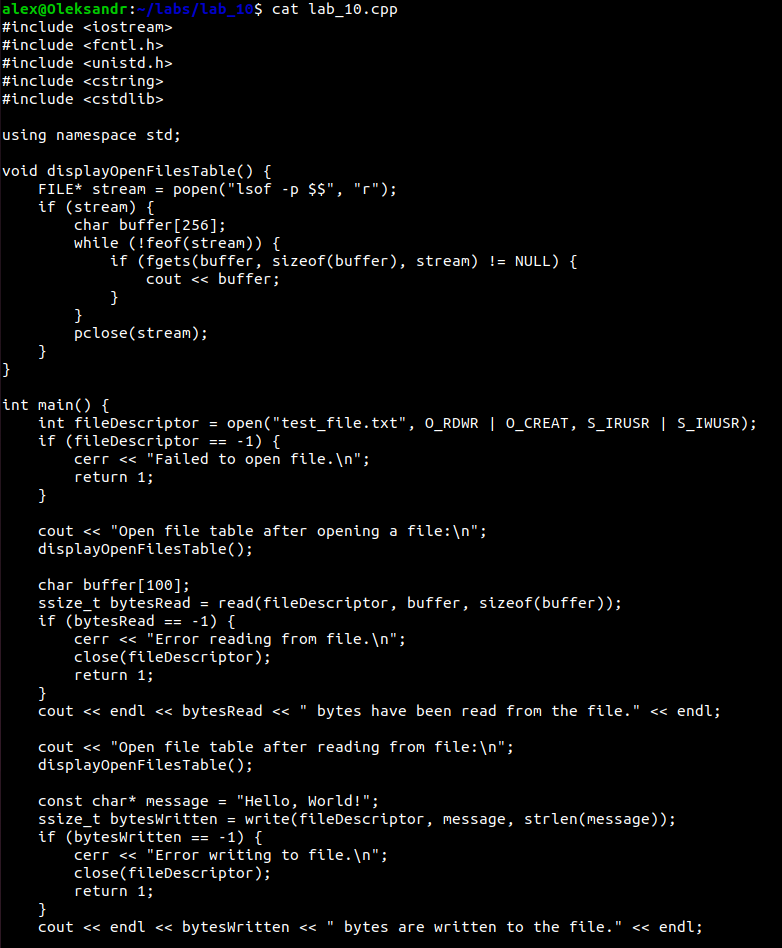
\includegraphics[width=0.8\linewidth]{Prt sc/Figure_1_1.png}  
        \end{minipage}
    \end{figure}
    \begin{figure}[h!]
        \begin{minipage}[h]{1\linewidth}
            \centering
            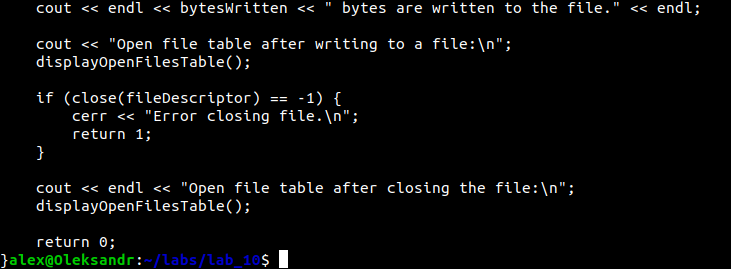
\includegraphics[width=0.8\linewidth]{Prt sc/Figure_1_2.png}  
        \end{minipage}
    \end{figure}

\newpage
    \begin{figure}[h!]
        \begin{minipage}[h]{1\linewidth}
            \centering
            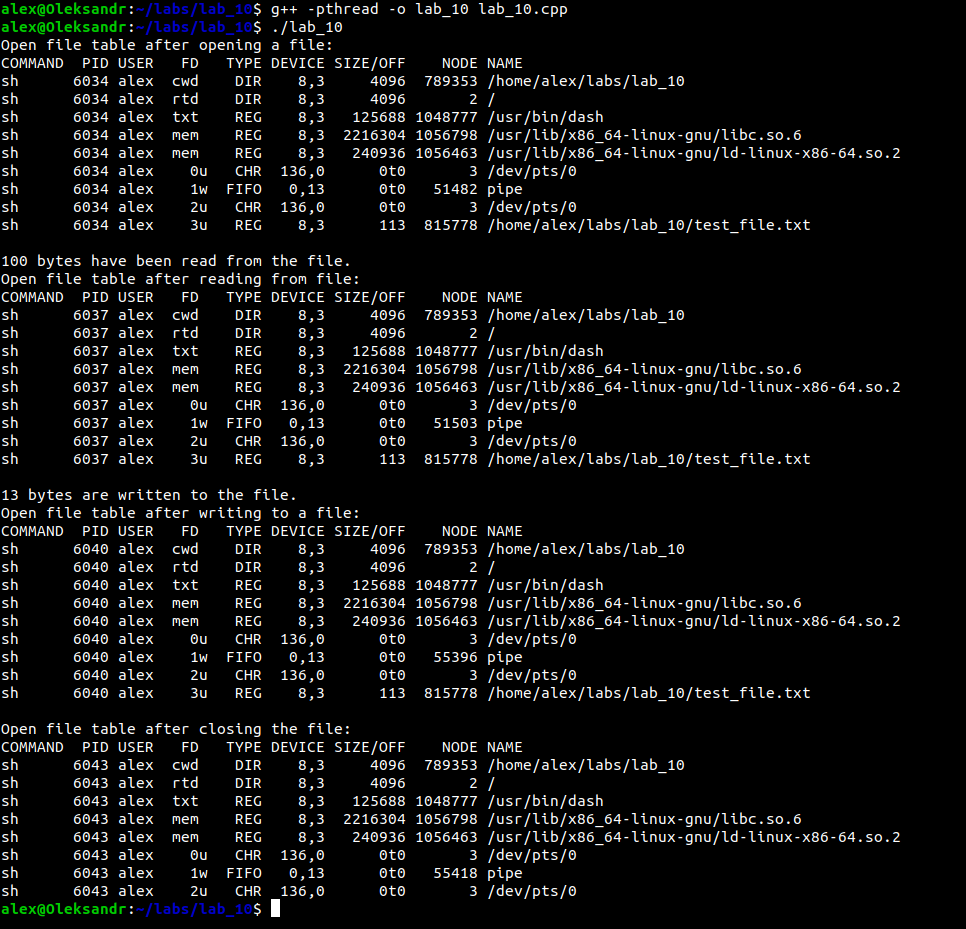
\includegraphics[width=0.8\linewidth]{Prt sc/Figure_2.png}  
        \end{minipage}
    \end{figure}
    \begin{center}
        \Large{Висновки}
    \end{center}

    Файлові системи забезпечують організацію та керування збереженням даних на диску. Linux підтримує різноманітні типи файлових систем, такі як ext4, XFS, Btrfs та інші.

    Віртуальна файлова система (VFS) забезпечує спільний інтерфейс для взаємодії з різними файловими системами. 
    Вона дозволяє програмам працювати з файлами та каталогами незалежно від конкретної файлової системи, що використовується. 
    Це робить розробку програм, які працюють з файловою системою, більш універсальною та зручною.

    Основними структурами даних для VFS є іноді (inode), файлова таблиця (file table) 
    та опис процесу (process descriptor). Іноди є структурою даних, яка містить інформацію про кожен файл або каталог. 
    Файлова таблиця зберігає відкриті файлові дескриптори та іншу інформацію про відкриті файли. Опис процесу містить інформацію про кожен активний процес в системі.

    Доступ до файлів здійснюється за допомогою системних викликів, таких як open, read, write, close і т.д. 
    Ці системні виклики дозволяють програмам взаємодіяти з файлами. Вони забезпечують стандартизований спосіб доступу до файлів незалежно від конкретної файлової системи.

    Тобто файлові системи в Linux є ключовим компонентом ОС і виконують важливі завдання з організації та управління файлами.

\end{document}